% \section{Normalization}\label{sec:norm}

% \section*{Database Schema}
% The following database schema is used in the campus event management system:

% \begin{itemize}
%     \item \textbf{department(department\_id, department\_name)}
%     \item \textbf{user(user\_id, username, email, password, user\_type, department\_id, contact\_number)}
%     \item \textbf{student(student\_id, enrollment\_date, user\_id)}
%     \item \textbf{teacher(teacher\_id, employment\_date, department\_id, user\_id)}
%     \item \textbf{location(location\_id, room\_number, building, capacity, is\_available)}
%     \item \textbf{event\_category(category\_id, category\_name)}
%     \item \textbf{event(event\_id, event\_name, description, event\_date, start\_time, end\_time, status, max\_attendees, currently\_registered, category\_id, location\_id)}
%     \item \textbf{registers(user\_id, event\_id, registration\_date)}
%     \item \textbf{organized\_by(user\_id, event\_id)}
% \end{itemize}

% \section*{Normalization Proof}

% \subsection*{First Normal Form (1NF)}
% To satisfy 1NF:
% \begin{itemize}
%     \item Each column must contain atomic (indivisible) values.
%     \item Each table must have a unique primary key.
% \end{itemize}

% \noindent \textbf{Proof:} Each table in the schema has atomic columns, with no repeating groups or arrays, and each row is uniquely identified by a primary key in each table. Therefore, the schema is in 1NF.

% \subsection*{Second Normal Form (2NF)}
% To satisfy 2NF:
% \begin{itemize}
%     \item The schema must be in 1NF.
%     \item All non-key attributes must depend on the whole primary key (no partial dependencies).
% \end{itemize}

% \noindent \textbf{Proof:} All tables with a single primary key automatically satisfy 2NF since there are no partial dependencies. Tables with composite primary keys (\textbf{registers} and \textbf{organized\_by}) also satisfy 2NF, as each non-key attribute depends on the entire composite primary key. Therefore, the schema is in 2NF.

% \subsection*{Third Normal Form (3NF)}
% To satisfy 3NF:
% \begin{itemize}
%     \item The schema must be in 2NF.
%     \item There should be no transitive dependencies, meaning non-key attributes must depend only on the primary key.
% \end{itemize}

% \noindent \textbf{Proof:} Each non-key attribute in each table depends only on the primary key:
% \begin{itemize}
%     \item In the \textbf{user} table, \texttt{department\_id} references the \textbf{department} table without any transitive dependencies, as departments are stored in a separate table.
%     \item In the \textbf{event} table, \texttt{category\_id} and \texttt{location\_id} reference separate tables (\textbf{event\_category} and \textbf{location}), avoiding any transitive dependencies.
% \end{itemize}
% Since each table in the schema is in 2NF and has no transitive dependencies, the schema is in 3NF.

% \subsection*{Boyce-Codd Normal Form (BCNF)}
% To satisfy BCNF:
% \begin{itemize}
%     \item The schema must be in 3NF.
%     \item Every determinant must be a candidate key.
% \end{itemize}

% \noindent \textbf{Proof:} In each table, there are no partial or transitive dependencies, and all non-key attributes depend solely on candidate keys. As such, the schema adheres to BCNF.

% \section*{Conclusion}
% The schema is normalized up to Boyce-Codd Normal Form (BCNF). Each table in the schema adheres to the requirements of 1NF, 2NF, 3NF, and BCNF, ensuring data integrity and eliminating redundancy.

% \clearpage



% \subsection{Normalization Analysis}

% \subsubsection{user Table}
% \begin{itemize}
%     \item \textbf{Primary Key:} username
%     \item \textbf{Functional Dependencies:} \texttt{username} $\rightarrow$ \texttt{name, email, password, user\_type, department, contact\_number}
%     \item \textbf{Normalization:}
%     \begin{itemize}
%         \item \textbf{3NF:} Each non-key attribute depends only on \texttt{username}, so it's in 3NF.
%         \item \textbf{BCNF:} Since \texttt{username} is the only candidate key, it is also in BCNF.
%     \end{itemize}
% \end{itemize}

% \subsubsection{student Table}
% \begin{itemize}
%     \item \textbf{Primary Key:} student\_id
%     \item \textbf{Functional Dependencies:} \texttt{student\_id} $\rightarrow$ \texttt{enrollment\_date, username}
%     \item \textbf{Normalization:}
%     \begin{itemize}
%         \item \textbf{3NF:} Each non-key attribute depends only on \texttt{student\_id}, so it's in 3NF.
%         \item \textbf{BCNF:} As \texttt{student\_id} is the only candidate key, it is also in BCNF.
%     \end{itemize}
% \end{itemize}

% \subsubsection{teacher Table}
% \begin{itemize}
%     \item \textbf{Primary Key:} teacher\_id
%     \item \textbf{Functional Dependencies:} \texttt{teacher\_id} $\rightarrow$ \texttt{employment\_date, username}
%     \item \textbf{Normalization:}
%     \begin{itemize}
%         \item \textbf{3NF:} Each non-key attribute depends only on \texttt{teacher\_id}, so it's in 3NF.
%         \item \textbf{BCNF:} With \texttt{teacher\_id} as the only candidate key, it is also in BCNF.
%     \end{itemize}
% \end{itemize}

% \subsubsection{location Table}
% \begin{itemize}
%     \item \textbf{Primary Key:} location\_id
%     \item \textbf{Functional Dependencies:} \texttt{location\_id} $\rightarrow$ \texttt{address, description, is\_available}
%     \item \textbf{Normalization:}
%     \begin{itemize}
%         \item \textbf{3NF:} Each non-key attribute depends only on \texttt{location\_id}, so it’s in 3NF.
%         \item \textbf{BCNF:} With \texttt{location\_id} as the only candidate key, it is also in BCNF.
%     \end{itemize}
% \end{itemize}

% \subsubsection{event Table}
% \begin{itemize}
%     \item \textbf{Primary Key:} event\_id
%     \item \textbf{Functional Dependencies:} \texttt{event\_id} $\rightarrow$ \texttt{event\_name, description, event\_date, start\_time, end\_time, status, max\_attendees, currently\_registered, category\_id, location\_id}
%     \item \textbf{Normalization:}
%     \begin{itemize}
%         \item \textbf{3NF:} Each non-key attribute depends only on \texttt{event\_id}, so it’s in 3NF.
%         \item \textbf{BCNF:} Since \texttt{event\_id} is the only candidate key, it is also in BCNF.
%     \end{itemize}
% \end{itemize}

% \subsubsection{registers Table}
% \begin{itemize}
%     \item \textbf{Primary Key:} (username, event\_id)
%     \item \textbf{Functional Dependencies:} (username, event\_id) $\rightarrow$ \texttt{registration\_date}
%     \item \textbf{Normalization:}
%     \begin{itemize}
%         \item \textbf{3NF:} Each non-key attribute depends only on the composite key (username, event\_id), so it’s in 3NF.
%         \item \textbf{BCNF:} There are no additional candidate keys, so it’s in BCNF.
%     \end{itemize}
% \end{itemize}

% \subsubsection{organized\_by Table}
% \begin{itemize}
%     \item \textbf{Primary Key:} (username, event\_id)
%     \item \textbf{Functional Dependencies:} (username, event\_id) $\rightarrow$ \texttt{None}
%     \item \textbf{Normalization:}
%     \begin{itemize}
%         \item \textbf{3NF and BCNF:} It’s a junction table with no non-key attributes, so it’s automatically in BCNF.
%     \end{itemize}
% \end{itemize}





\section{Normalization of Database Tables}

Normalization is a process used to minimize or remove data redundancy in a set of relations. The primary goal of normalization is to eliminate anomalies that can occur during data insertion, update, or deletion, thus making the database consistent, dependency-preserving, and free of redundancy. Below, we analyze the normalization forms (specifically 3NF) for each table in the campus event management database.

\subsection{Normalizing user Table}

The \texttt{user} table has the attributes:
\[
\{ \texttt{username}, \texttt{name}, \texttt{email}, \texttt{password}, \texttt{user\_type}, \texttt{contact\_number} \}
\]
\begin{figure}[h]
    \centering
    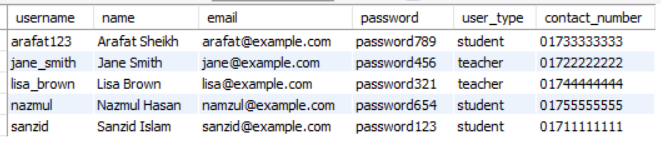
\includegraphics[scale=0.7]{images/table_data/user_table.png}
\end{figure}
% \csvautotabular{table_data/user.csv}

% \pgfplotstabletypeset[
%     col sep=comma, % Define column separator
%     header=true, % Use the first row as headers
%     every head row/.style={before row=\hline, after row=\hline}, % Add horizontal lines
%     every last row/.style={after row=\hline}
% ]{table_data/user.csv} 


Based on the demo data, we identify the following functional dependencies and analyze the candidate keys, 
prime attributes, and non-prime attributes to determine its normalization status.

\begin{itemize}
    \item \textbf{Functional Dependencies:}
    \begin{itemize}
        \item \texttt{\underline{username}} $\rightarrow$ \texttt{username,name, email, password, user\_type, contact\_number}
    \end{itemize}
    \begin{itemize}
        \item \texttt{email}$\rightarrow$ \texttt{username,name, email, password, user\_type, contact\_number}
    \end{itemize}
    \begin{itemize}
        \item \texttt{contact\_number} $\rightarrow$ \texttt{username,name, email, password, user\_type, contact\_number}
    \end{itemize}



    \item \textbf{Candidate Keys:} \texttt{username, email, contact\_number}
    
    \item \textbf{Prime Attributes:} \texttt{username,email, contact\_number}

    \item \textbf{Non-Prime Attributes:} \texttt{name, password, user\_type}

    \item \textbf{Analysis:} Based on our analysis, all the functional dependencies in the \texttt{user} table have a candidate key on the left-hand side. This satisfies the requirements of 3NF, and no transitive dependencies are present. All non-prime attributes (name, email, password, user\_type, department, and contact\_number) are fully functionally dependent on the candidate key, \texttt{username}.

    \item \textbf{Conclusion:} The \texttt{user} table is in 3NF.
\end{itemize}

\subsection{Normalizing student Table}

The \texttt{student} table has the attributes:
\[
\{ \texttt{student\_id}, \texttt{enrollment\_date}, \texttt{username} \}
\]
\begin{figure}
    [h]
    \centering
    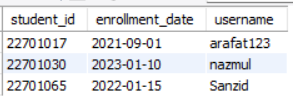
\includegraphics{images/table_data/student_table (1).png}
\end{figure}
\begin{itemize}
    \item \textbf{Functional Dependencies:}
    \begin{itemize}
        \item \texttt{student\_id} $\rightarrow$ \texttt{enrollment\_date, username}
    \end{itemize}

    \item \textbf{Candidate Keys:} \texttt{student\_id}

    \item \textbf{Prime Attributes:} \texttt{student\_id}

    \item \textbf{Non-Prime Attributes:} \texttt{enrollment\_date, username}

    \item \textbf{Analysis:} In this table, all functional dependencies have a candidate key on the left-hand side, fulfilling the conditions of 3NF. There are no transitive dependencies, and all non-prime attributes are fully functionally dependent on \texttt{student\_id}.

    \item \textbf{Conclusion:} The \texttt{student} table is in 3NF.
\end{itemize}

\subsection{Normalizing teacher Table}

The \texttt{teacher} table has the attributes:
\[
\{ \texttt{teacher\_id}, \texttt{employment\_date}, \texttt{username} \}
\]
\begin{figure}
    [h]
    \centering
    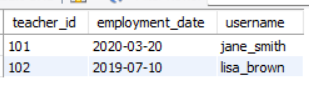
\includegraphics{images/table_data/teacher_table.png}
\end{figure}
\begin{itemize}
    \item \textbf{Functional Dependencies:}
    \begin{itemize}
        \item \texttt{teacher\_id} $\rightarrow$ \texttt{employment\_date, username}
    \end{itemize}

    \item \textbf{Candidate Keys:} \texttt{teacher\_id}

    \item \textbf{Prime Attributes:} \texttt{teacher\_id}

    \item \textbf{Non-Prime Attributes:} \texttt{employment\_date, username}

    \item \textbf{Analysis:} This table meets the conditions of 3NF as all functional dependencies have a candidate key on the left-hand side. There are no transitive dependencies, and all non-prime attributes are fully functionally dependent on \texttt{teacher\_id}.

    \item \textbf{Conclusion:} The \texttt{teacher} table is in 3NF.
\end{itemize}

\subsection{Normalizing venue Table}

The \texttt{venue} table has the attributes:
\[
\{ \texttt{venue\_id}, \texttt{venue\_name} , \texttt{location\_id}\}
\]
\begin{figure}
    [h]
    \centering
    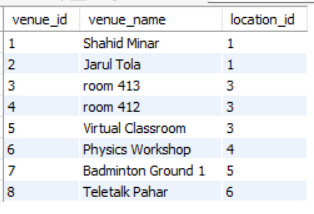
\includegraphics{images/table_data/venue_table.png}
\end{figure}
\begin{itemize}
    \item \textbf{Functional Dependencies:}
    \begin{itemize}
        \item \texttt{venue\_id} $\rightarrow$ \texttt{venue\_name, location\_id}
    \end{itemize}

    \item \textbf{Candidate Keys:} \texttt{venue\_id}

    \item \textbf{Prime Attributes:} \texttt{venue\_id}

    \item \textbf{Non-Prime Attributes:} \texttt{venue\_name,location\_id}

    \item \textbf{Analysis:} The functional dependency has a candidate key 
    (\texttt{venue\_id}) on the left-hand side. This satisfies the conditions of 3NF, 
    and there are no transitive dependencies. All non-prime attributes 
    (\texttt{venue\_name,location\_id}) are fully functionally dependent on \texttt{venue\_id}.

    \item \textbf{Conclusion:} The \texttt{venue} table is in 3NF.
\end{itemize}



\subsection{Normalizing location Table}

The \texttt{location} table has the attributes:
\[
\{ \texttt{location\_id}, \texttt{location\_name} \}
\]
\begin{figure}
    [h]
    \centering
    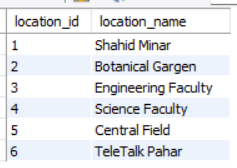
\includegraphics{images/table_data/location_table.png}
\end{figure}
\begin{itemize}
    \item \textbf{Functional Dependencies:}
    \begin{itemize}
        \item \texttt{location\_id} $\rightarrow$ \texttt{location\_name}
    \end{itemize}

    \item \textbf{Candidate Keys:} \texttt{location\_id}

    \item \textbf{Prime Attributes:} \texttt{location\_id}

    \item \textbf{Non-Prime Attributes:} \texttt{location\_name}

    \item \textbf{Analysis:} The functional dependency has a candidate key 
    (\texttt{location\_id}) on the left-hand side. This satisfies the conditions of 3NF, 
    and there are no transitive dependencies. All non-prime attributes 
    (\texttt{location\_name}) are fully functionally dependent on \texttt{location\_id}.

    \item \textbf{Conclusion:} The \texttt{location} table is in 3NF.
\end{itemize}

\subsection{Normalizing event\_category Table}

The \texttt{event\_category} table has the attributes:
\[
\{ \texttt{category\_id}, \texttt{category\_name} \}
\]
\begin{figure}
    [h]
    \centering
    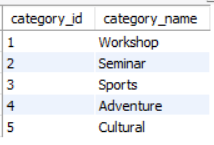
\includegraphics{images/table_data/event_category.png}
\end{figure}
\begin{itemize}
    \item \textbf{Functional Dependencies:}
    \begin{itemize}
        \item \texttt{category\_id} $\rightarrow$ \texttt{category\_name}
    \end{itemize}

    \item \textbf{Candidate Keys:} \texttt{category\_id}

    \item \textbf{Prime Attributes:} \texttt{category\_id}

    \item \textbf{Non-Prime Attributes:} \texttt{category\_name}

    \item \textbf{Analysis:} The functional dependency has a candidate key (\texttt{category\_id}) on the left-hand side, meeting 3NF requirements. There are no transitive dependencies, and all non-prime attributes are fully functionally dependent on \texttt{category\_id}.

    \item \textbf{Conclusion:} The \texttt{event\_category} table is in 3NF.
\end{itemize}

\subsection{Normalizing event Table}

The \texttt{event} table has the attributes:
\[
\{ \texttt{event\_id}, \texttt{event\_name}, \texttt{description}, \texttt{event\_date}, \texttt{start\_time}, \texttt{end\_time}, \texttt{status}, \texttt{max\_attendees}, \texttt{category\_id}, \texttt{venue\_id} \}
\]

\begin{figure}
    [h]
    \centering
    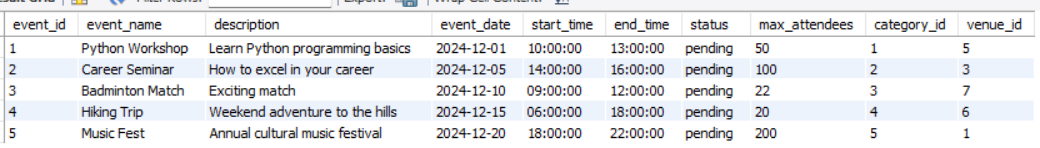
\includegraphics{images/table_data/event.png}
\end{figure}

\begin{itemize}
    \item \textbf{Functional Dependencies:}
    \begin{itemize}
        \item \texttt{event\_id} $\rightarrow$ \texttt{event\_name, description, event\_date, start\_time, end\_time, status, max\_attendees, category\_id, venue\_id}
    \end{itemize}

    \item \textbf{Candidate Keys:} \texttt{event\_id}

    \item \textbf{Prime Attributes:} \texttt{event\_id}

    \item \textbf{Non-Prime Attributes:} \texttt{event\_name, description, event\_date, start\_time, end\_time, status, max\_attendees, category\_id, venue\_id}

    \item \textbf{Analysis:} All functional dependencies have a candidate key (\texttt{event\_id}) on the left-hand side. There are no transitive dependencies, and all non-prime attributes are fully functionally dependent on \texttt{event\_id}, fulfilling 3NF.

    \item \textbf{Conclusion:} The \texttt{event} table is in 3NF.
\end{itemize}

\subsection{Normalizing registers Table}

The \texttt{registers} table has the attributes:
\[
\{ \texttt{username}, \texttt{event\_id}, \texttt{registration\_date} \}
\]

\begin{itemize}
    \item \textbf{Functional Dependencies:}
    \begin{itemize}
        \item \texttt{(username, event\_id)} $\rightarrow$ \texttt{registration\_date}
    \end{itemize}

    \item \textbf{Candidate Keys:} \texttt{(username, event\_id)}

    \item \textbf{Prime Attributes:} \texttt{username, event\_id}

    \item \textbf{Non-Prime Attributes:} \texttt{registration\_date}

    \item \textbf{Analysis:} The only functional dependency has a composite candidate key (\texttt{username, event\_id}) on the left-hand side, fulfilling 3NF. There are no transitive dependencies, and the non-prime attribute \texttt{registration\_date} is fully functionally dependent on the composite key.

    \item \textbf{Conclusion:} The \texttt{registers} table is in 3NF.
\end{itemize}

\subsection{Normalizing organized\_by Table}

The \texttt{organized\_by} table has the attributes:
\[
\{ \texttt{username}, \texttt{event\_id} \}
\]

\begin{itemize}
    \item \textbf{Functional Dependencies:}
    \begin{itemize}
        \item \texttt{(username, event\_id)} $\rightarrow$ \texttt{[no additional attributes]}
    \end{itemize}

    \item \textbf{Candidate Keys:} \texttt{(username, event\_id)}

    \item \textbf{Prime Attributes:} \texttt{username, event\_id}

    \item \textbf{Non-Prime Attributes:} None

    \item \textbf{Analysis:} The table consists only of the composite candidate key (\texttt{username, event\_id}), so there are no additional attributes to check for dependency. Thus, it satisfies 3NF.

    \item \textbf{Conclusion:} The \texttt{organized\_by} table is in 3NF.
\end{itemize}

